\section{案例研究:对DVD加密系统的密码学分析}

内容加扰系统(Content Scrambling System, CSS)是一个用于保护DVD光盘上电影的系统。它使用一种称为CSS的流密码来加密电影内容。CSS设计于20世纪80年代,当时,可出口的加密算法被限制在$40$比特密钥以内。因此,CSS使用$40$比特的密钥对电影进行加密。虽然我们现在已经知道,使用$40$比特密钥的密码是非常不安全的,但我们将表明,CSS流密码格外弱,以至于我们可以找到比穷举所有$2^{40}$个密钥耗时更短的破解方法。它为密码分析提供了一个有趣的机会。

\begin{snote}[线性反馈移位寄存器(Linear feedback shift register, LFSR)。]
CSS流密码由两个LFSR构建。一个$n$比特LFSR由一组整数$V:=\{v_1,\dots,v_d\}$定义,其中每个$v_i$都在$\{0,\dots,n-1\}$中。$V$中的元素被称为\textbf{抽头位置(tap position)}。一个LFSR能够提供一个PRG(见图 \ref{fig:3-10}),其原理如下所示:

\vspace*{5pt}

\hspace*{5pt} 输入:$s=(b_{n-1},\dots,n_0)\in\{0,1\}^n$,其中$s\neq 0^n$\\
\hspace*{26pt} 输出:$y\in\{0,1\}^\ell$,其中$\ell>n$\\
\hspace*{26pt} 对于 $i\leftarrow1$ 到 $\ell$:\\
\hspace*{26pt} \quad\quad\quad 输出 $b_0$ \hspace*{81.5pt} // \emph{输出一比特}\\
\hspace*{26pt} \quad\quad\quad $b\leftarrow b_{v_1}\oplus\cdots\oplus b_{v_d}$ \hspace*{29.5pt} // \emph{计算反馈比特}\\
\hspace*{26pt} \quad\quad\quad $s\leftarrow(b,b_{n-1},\dots,b_1)$ \hspace*{23pt} // \emph{将寄存器中的比特右移}

\vspace*{5pt}

\noindent
LFSR每个时钟周期输出一个比特。请注意,如果一个LFSR在启动时状态为$s=0^n$,那么它的输出会退化为全部是$0$。由于这个原因,种子中的某一比特必须总是被置为$1$。

LFSR可以用很少的晶体管在硬件上实现。因此,由LFSR构建的流密码对于低成本的消费电子产品(如DVD播放器、手机和蓝牙设备)很有吸引力。
\end{snote}

\begin{figure}
  \centering
  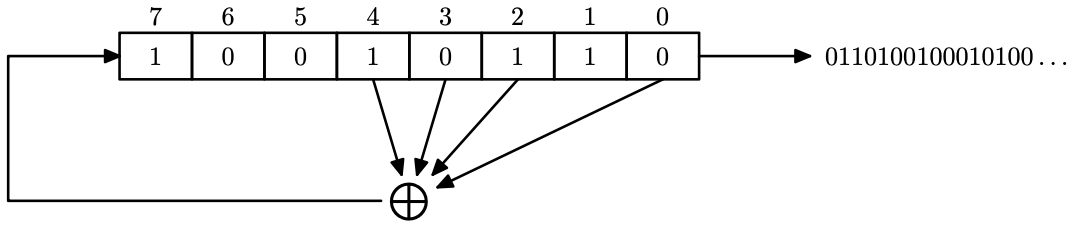
\includegraphics[width=0.7\linewidth]{figures/chapter3/fig10.png}
  \caption{$8$比特的线性反馈移位寄存器$\{4,3,2,0\}$}
  \label{fig:3-10}
\end{figure}

\begin{snote}[来自LSFR的流密码。]
一个单一的LFSR作为PRG是完全不安全的,因为给定其输出的$n$个连续比特,很容易就能计算出所有的后续比特。然而,使用一个非线性组件把几个LFSR组合起来,我们就有可能得到在某种程度上(弱)安全的PRG。一种属于eStream组合的流密码 Trivium 就是这样构建出来的。

从 LFSR 构建流密码的一种方法是并行地运行几个 LFSR,并使用非线性操作组合它们的输出。接下来描述的CSS流密码使用整数域上的加法将两个 LFSR 组合起来。而被用于加密 GSM 手机流量的 A5/1 流密码组合了三个 LFSR 的输出。蓝牙 E0 流密码使用一个 $2$ 比特的有限状态机将四个 LFSR 组合起来。所有这些算法都已被证明是不安全的,并且不应该被使用,这是因为对于这些密码,恢复明文所需的时间远远少于对密钥空间进行穷举搜索的耗时。

另一种方法是只运行一个 LFSR,并对其内部状态进行非线性操作来产生输出。用于加密 3GPP 手机流量的 \texttt{snow} 3G 密码就是这样操作的。
\end{snote}

\begin{snote}[CSS流密码。]
CSS流密码是由图 \ref{fig:3-11} 所示的 PRG 建立的。该 PRG 的工作原理如下:

\vspace*{5pt}

\hspace*{5pt} 输入:种子 $s\in\{0,1\}^{40}$\\
\hspace*{26pt} 输出:$\ell$ 个比特

\vspace{3pt}

\hspace*{5pt} 令 $s=s_1 \Vert s_2$,其中 $s_1\in\{0,1\}^{16}$,$s_2\in\{0,1\}^{24}$\\
\hspace*{26pt} 将 $1\Vert s_1$ 加载到一个 $17$ 比特的 LFSR 中\\
\hspace*{26pt} 将 $1\Vert s_2$ 加载到一个 $25$ 比特的 LFSR 中\\
\hspace*{26pt} 令 $c\leftarrow 0$ \quad\quad // \emph{进位}\\
\hspace*{26pt} 对于 $i=1,\dots,\ell$:\\
\hspace*{50pt} 将两个 LFSR 运行 $8$ 个周期,得到 $x_i,y_i\in\{0,1\}^8$\\
\hspace*{50pt} 将 $x_i$ 和 $y_i$ 视作 $\{0,\dots,255\}$ 中的两个整数\\
\hspace*{50pt} 输出 $z_i:=x_i+y_i+c\;\mathrm{mod}\;256$\\
\hspace*{50pt} 如果 $x_i+y_i>255$,则令 $c\leftarrow1$,否则令 $c\leftarrow0$ \quad\quad // \emph{进位}

\vspace*{5pt}

该 PRG 每次迭代输出一个字节。在 $s_1$ 和 $s_2$ 中预留的 $1$ 确保 LFSR 不会被初始化为全 $0$ 状态。两个 LFSR 的抽头是固定的。$17$ 比特的 LFSR 使用的是抽头 $\{14,0\}$,25比特的 LFSR 使用抽头 $\{12,4,3,0\}$。

我们展示的 CSS PRG 是 CSS 的一个小变体,它描述起来比较容易,但和真正的 CSS 具有同等的安全性。在真正的 CSS 中,对于 $17$ 比特的 LFSR,我们不是在初始种子中预置 $1$,而是在第 $9$ 比特的位置插入 $1$;而对于 $25$ 比特的 LFSR,是在第 $22$ 比特处插入 $1$。此外,真正的 CSS 会丢弃 $17$ 比特 LFSR 输出的第一个字节和 $25$ 比特 LFSR 输出的前两个字节。这两个问题都不会影响到接下来的分析。
\end{snote}

\begin{figure}
  \centering
  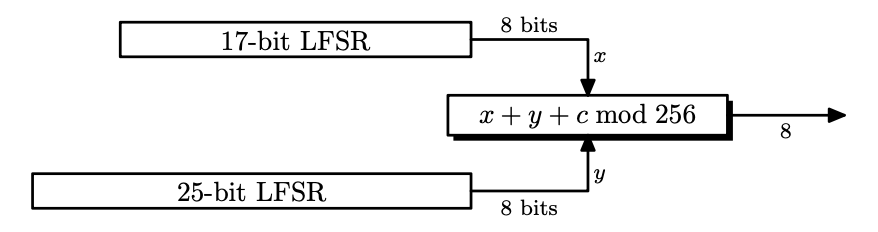
\includegraphics[width=0.6\linewidth]{figures/chapter3/fig11.png}
  \caption{CSS流密码}
  \label{fig:3-11}
\end{figure}

\begin{snote}[CSS的不安全性。]
给定一个 PRG 的输出,通过对种子空间进行穷举搜索,我们显然可以在 $2^{40}$ 次计算内恢复秘密的种子。我们下面展示一种更快的攻击方法,它只需要进行 $2^{16}$ 次猜测。假设我们得到了 PRG 输出的前 $100$ 个字节 $\bar{z}:=(z_1,z_2,\dots)$。该攻击基于以下观察:
\begin{quote}
令 $(x_1,x_2,x_3)$ 和 $(y_1,y_2,y_3)$ 分别为 $17$ 比特和 $25$ 比特的 LFSR 所输出的前三个字节。那么:
\[
(2^{16}x_3+2^8x_2+x_1)+(2^{16}y_3+2^8y_2+y_1)\equiv(2^{16}z_3+2^8z_2+z_1)\quad(\mathrm{mod}\;2^{24})
\]
因此,一旦 $(z_1,z_2,z_3)$ 和 $(x_1,x_2,x_3)$ 都已经知道了,我们就可以很容易地计算出 $(y_1,y_2,y_3)$,进而可以很容易地得到 $25$ 比特的 LFSR 的初始状态 $s_2$。
\end{quote}
有了这个观察,攻击者就可以通过尝试所有可能的 $16$ 比特的 $s_1$ 的值来恢复种子 $s$。对于每个猜测的 $s_1$,它计算出 $17$ 比特 LFSR 对应的输出 $(x_1,x_2,x_3)$。利用上面的观察,它就能够获得一个 $25$ 比特 LFSR 的候选种子 $s_2$。然后,为了确认 $\hat{s}:=s_1\Vert s_2$ 是否是正确的秘密种子,它使用种子 $\hat{s}$ 运行 PRG 的 $100$ 次迭代,并将输出的结果与给定的序列 $\bar{z}$ 进行比较。如果序列不匹配,就换一个 $s_1$ 重新进行计算。一旦攻击者找到了正确的 $s_1$,生成的序列将与给定的 $\bar{z}$ 相匹配,在这种情况下,攻击者就得到了正确的秘密种子 $\hat{s}:=s_1\Vert s_2$。

我们上面的分析表明,在期望上对 $s_1$ 进行 $2^{15}$ 次猜测后,就可以找到整个种子 $s$。这比单纯地进行 $2^{40}$ 次穷举搜索攻击要快得多。
\end{snote}